\documentclass[cap,cs5size,nospace,indent,fancyhdr]{ctexart}
\usepackage{booktabs}
\usepackage{caption}  
\usepackage{changepage}
\usepackage{geometry}
 \usepackage{pgfplots}
 \usepgfplotslibrary{dateplot}
\geometry{top=2cm,bottom=2cm}
\usepackage{tcolorbox}
\usepackage{xpinyin}
\usepackage{subfigure}
\usepackage{float}
\usepackage[T1]{fontenc}
\usepackage[utf8]{inputenc}
\usepackage{authblk}

\title{Math 286 Lab Project}
\date{2020, Sept, 11th}
\author{\textbf{Ruan Yucheng} 3180111}
\author{\textbf{Zhang Zheyuan} 3180111607}
\author{\textbf{Wu Zheyu} 3180111}
\author{\textbf{Qian Chen} 3180111591}
\author{\textbf{Zheng Xiuwen} 3180111}
\affil{Department of Mechanical Engineering, ZJUI}
\renewcommand\Authands{ and }

\begin{document}
\maketitle

Determine the maximal solution of the following ODE with the initial value.

\begin{equation}
	y' = t^2+y^3, y(0)=1
\end{equation}

\section{Problem 1}
\subsection{Direction Field}
At first, we plot the direction field of (1). After connecting the direction arrows we find that the curve seems has 2 vertical asymptotes, which approximately lies between -2.1 to -2.2 and 0.8 to 0.9.

\begin{center}
	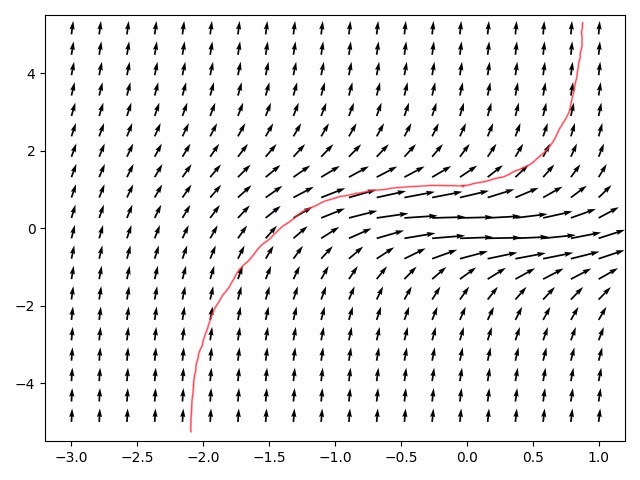
\includegraphics[scale=0.3]{HandSketch.jpeg}
\end{center}

\subsection{Numerical Methods}

\subsubsection{Rough Approximation}
Firtly, we define: 

\[f(t,y) = y^2+t*y+t^2\]

Then we apply the formulas:
\[f_n = f(t_n, y_n)\]
\[y_{n+1} = y)n + h*f_n\]
\[t_{n+1} = t_n + h\]

By choosing step of $h = 0.1$, we cound obtain the table below:
\begin{table}
	\begin{center}
		\begin{tabular}{l|r|r|r|r|r|r|r|r}
			\textbf{T} & \textbf{-2.4} & \textbf{-2.3} & \textbf{-2.2} & \textbf{-2.1} & \textbf{0.8} & \textbf{0.9} & \textbf{1.0} & \textbf{1.1} \\

			y & -64.4655 & -19.8728 & -9.1019 & -5.0501 & 4.85430 & 7.6631 & 14.3061 & 36.3031 \\
			
		\end{tabular}
	\end{center}
	
\end{table}


\end{document}